% Nejprve uvedeme tridu dokumentu s volbami
\documentclass[czech,master,public,dept460,male,cpdeclaration,twoside]{diploma}
% Dalsi doplnujici baliky maker
\usepackage{subfig}		% makra pro "podobrazky" a "podtabulky"
\usepackage{tikz}		% makra pro kresleni

\usepackage{float}
\usepackage{color}

%javascript
\usepackage{listings}
\usepackage{color}
\definecolor{lightgray}{rgb}{.9,.9,.9}
\definecolor{darkgray}{rgb}{.4,.4,.4}
\definecolor{purple}{rgb}{0.65, 0.12, 0.82}

\lstdefinelanguage{JavaScript}{
  keywords={typeof, new, true, false, catch, function, return, null, catch, switch, var, if, in, while, do, else, case, break},
  keywordstyle=\color{blue}\bfseries,
  ndkeywords={class, export, boolean, throw, implements, import, this},
  ndkeywordstyle=\color{darkgray}\bfseries,
  identifierstyle=\color{black},
  sensitive=false,
  comment=[l]{//},
  morecomment=[s]{/*}{*/},
  commentstyle=\color{purple}\ttfamily,
  stringstyle=\color{red}\ttfamily,
  morestring=[b]',
  morestring=[b]"
}

\lstset{
   basicstyle=\tiny,
   xleftmargin=0.8cm,
   language=JavaScript,
   extendedchars=true,
   basicstyle=\footnotesize\ttfamily,
   showstringspaces=false,
   showspaces=false,
   numbers=left,
   numberstyle=\footnotesize,
   numbersep=9pt,
   tabsize=2,
   breaklines=true,
   showtabs=false,
   captionpos=b
}

\definecolor{gray}{rgb}{0.4,0.4,0.4}
\definecolor{darkblue}{rgb}{0.0,0.0,0.6}
\definecolor{cyan}{rgb}{0.0,0.6,0.6}

\lstdefinelanguage{XML}
{
  morestring=[b]",
  morestring=[s]{>}{<},
  morecomment=[s]{<?}{?>},
  stringstyle=\color{black},
  identifierstyle=\color{darkblue},
  keywordstyle=\color{cyan},
  morekeywords={xmlns,version,type}% list your attributes here
}

% Zadame pozadovane vstupy pro generovani titulnich stran.
\ThesisAuthor{Jan Čech}

\CzechThesisTitle{Bakalářská práce - Hra Port Royal a moderní vývoj softwaru}

\EnglishThesisTitle{Bachelor thesis - Game Port Royal and modern software development}

\SubmissionDate{20. dubna 2017}

% Pokud nechceme nikomu dekovat makro zapoznamkujeme.
\Thanks{Rád bych na tomto místě poděkoval Ing. Davidovi Ježkovi, Ph.D., za pomoc a vedení u této práce.}

% Zadame cestu a jmeno souboru ci nekolika souboru s digitalizovanou podobou zadani prace.
% Pokud toto makro zapoznamkujeme sazi se stranka s upozornenim.
\ThesisAssignmentImagePath{Figures/zadani}

% Zadame soubor s digitalizovanou podobou prohlaseni autora zaverecne prace.
% Pokud toto makro zapoznamkujeme sazi se cisty text prohlaseni.
\AuthorDeclarationImageFile{Figures/samostatne.jpg}

\CooperatingPersonsDeclarationImageFile{Figures/zverejneni.jpg}

\CzechAbstract{Cílem této práce bylo prozkoumat použití moderních technologií pro vývoj webových aplikací včetně technologií pro jejich testování. Praktická část obsahuje webovou aplikaci, jež je vytvořena pomocí technologií Spring a AngulaJS, ty spolu komunikují přes rozhraní podle architektury REST. Tato aplikace je testována pomocí technologii Jasnime, Protractor a Jersey. Všechny zmíněné technologie jsou popsány v teoretické části práce.}

\CzechKeywords{diplomová práce, AngularJS, Spring, Jasmine, Protractor, Jersey, moderní web, testování softwaru}

\EnglishAbstract{The aim of this thesis is examine usage of modern technologies for development web applivations, include technologies for their testing. Practical part contains an application developed by dint of Spring and AngulaJS technologies. The communication of those two technologies is based on REST architecture. This application is tested on Jasmine, Protractor and Jersey technologies. All these technologies are described in theoretical part of this thesis.}

\EnglishKeywords{master thesis, AngularJS, Spring, Jasmine, Protractor, Jersey, modern web, software testing}

\AddAcronym{REST}{REpresentational State Transfer}
\AddAcronym{HTML}{Hyper Text Markup Language}
\AddAcronym{XML}{Extensible Markup Language}
\AddAcronym{JSON}{JavaScript Object Notation}
\AddAcronym{J2EE}{Java 2 Platform, Enterprise Edition}
\AddAcronym{URI}{Uniform Resource Identifier}
\AddAcronym{URL}{Uniform Resource Locator}
\AddAcronym{TDD}{Test-driven development}
\AddAcronym{CSS}{Cascading Style Sheets}


% Zacatek dokumentu
\begin{document}

% Nechame vysazet titulni strany.
\MakeTitlePages

% Pokud mame v zaverecne praci vypisy kodu, jinak odstranit.
\lstlistoflistings

% A nasleduje text zaverecne prace.
\section{Úvod}
Jako vše v oblasti informačních technologií, v tak i oblasti vývoje webových stránek se objevuje spousta nových trendů. Tyto trendy se týkají jak nových technologií, jež usnadňují vývoj, tak také návrhu celé architektury aplikace, která vývoj zpřehledňuje a usnadňuje rozšířitelnost aplikace do budoucna. Také se do popředí dostává testování softwaru, jenž bylo kdysi okrajovou záležitostí. V dnešní době se však již stalo testování softwaru, standardní součástí vývoje aplikace. Zadáním této práce bylo všechny tyto trendy zachytit. Práce by se dala shrnout takto. Nejprve bylo nutno nastudovat moderní webové technologie Spring, AngularJS a REST architekturu, poté navrhnout a implementovat hru Port Royal. Následně nastudovat principy testování a vybrat technologie pro otestování vyvinuté aplikace. Nakonec ve vybraných technologiích otestovat aplikaci.


\subsection{Stručný obsah jednotlivých kapitol}
V následující 2. kapitole jsou popsány technologie pro vývoj webových aplikací. 3. kapitola se věnuje testování a technologiím zaměřeným na testování. Ve 4. kapitole je ukázána aplikace a popsány některé její technologické prvky. V 5. kapitole jsou popsány technologie pro vývoj webových aplikací z praktického hlediska a v 6. kapitole jsou více popsány testovací technologie, a to také z praktického hlediska. V poslední 7. kapitole je shrnutí bakalářské práce.

\section{Technologie}

\subsection{REST}
{\bf RE}presentational {\bf S}tate {\bf T}ransfer neboli REST představil Roy Fielding roku 2000 ve své disertační práci "Architectural Styles and the Design of Network-based Software Architectures". Tato architektura nemá žádné předchozí omezení,	 plní pouze následující architektonické požadavky:
\begin{itemize}
	\item \underline{Komunikace je klient-server} - Díky rozdělení na tyto dvě části se může klientská i serverová část vyvíjet nezávisle na té druhé. Také se takto umožní aby, klientská část fungovala na více platformách a je zbavená starosti o uložení dat.
	\item \underline{Bezstavovost} - Každý dotaz z klientské strany musí obsahovat všechny informace potřebné k jeho zpracování a nesmí využít žádný uložený kontext. Pokud je nutno držet nějaký stav, děje se to vždy na straně klienta. Díky této vlastnosti si server nemusí držet v paměti žádný stav, což zvyšuje jeho výkon. Na druhou stranu se tím zvyšuje objem přenesených dat mezi serverem a klientem.
	\item \underline{Uložitelnost do krátkodobé paměti} - Odpovědi serveru na dotazy by měly být označeny zda jsou uložitelné do krátkodobé paměti. Mnohdy se klient může ptát několikrát na stejný dotaz. Pokud se neočekává, že se odpověď bude měnit, je výhodné odpověď uložit do paměti. Takto je možné omezit zbytečnou komunikaci mezi serverem a klientem.
	\item \underline{Jednotné rozhraní} - REST má mít jednotné rozhraní, což usnadňuje orientaci v něm a zvyšuje rozšiřitelnost do budoucna. REST nemá určený typ media, metody ani syntaxi koncových bodů. Tudíž dotaz může být ve formátu XML, JSON, ale také například i ve formátu PDF. Přes různé protokoly a ne jenom přes webové URL.

Nejčastěji se však používá webové rozhraní s HTTP metodami. Tabulka~"Vzorové REST rozhraní"~ukazuje vzorové rozhraní, podobné tomu použitému v praktické části. POST se zde používá pro vytvářená záznamu, GET pro získání záznamu, PUT pro úpravu záznamů a DELETE pro mazání.\cite{RESTInterface}

\begin{table}[H]
	\centering
	\caption{Vzorové REST rozhraní}
	\label{tab:REST}
	\begin{tabular}{|c|c|c|}
		\hline
		{\bf HTTP metoda} & {\bf URI} & {\bf Operace} \\
		\hline
		GET & /administrace/uzivatele & Vrátí list všech uživatelů \\
		\hline
		GET & /administrace/uzivatele/1 & Vrátí data uživatele s ID 1 \\
		\hline
		POST & /administrace/uzivatele & Vloží nového uživatele \\
		\hline
		PUT & /administrace/uzivatele/1 & Upraví údaje uživatele s ID 1 \\
		\hline
		DELETE & /administrace/uzivatele/1 & Smaže uživatele s ID 1 \\
		\hline
	\end{tabular}
\end{table}
	\item \underline{Vrstvený systém} - mezi klientem a serverem mohou být různé vrstvy neboli prostřednici. U těchto vrstev platí, že každá vrstva ví pouze o vrstvě, jež následuje bezprostředně po ní. Další vrstvy a celá architektura zůstávají skryté, aby se zajistila nezávislost vrstev. Touto vrstvou může být firewall nebo obalení historické vrstvy za účelem přidání nové funkcionality. 
	\item \underline{Kód na vyžádání} - Tato vlastnost není povinná. Jedná se o to, že klient může mít schopnost stáhnout si kód ze serverové strany, například plugin do prohlížeče nebo kód v jazyce JavaScript. Tato schopnost se hodí pokud je možno provádět serverovou logiku lépe na straně prohlížeče.
\end{itemize} \cite{RESTWebServicesOracle} \cite{RESTWebServicesOracle2}
	
\subsection{AngularJs}
AngularJS je javascriptový rámec založen na model-view-controller architektuře, určený pro vývoj jednostránkových aplikací. AngularJS rozšiřuje HTML direktivy, používá dvoucestný databinding a dependency injection, je u něj vysoká znovupoužitelnost komponentů. Celkově tak usnadňuje a urychluje vývoj webové části aplikace. Pro přístup na serverovou část využívá AngularJS webové služby. Všechny jeho výše zmíněné prvky jsou popsány v následujících podkapitolách. \cite{coJeAngular}

\subsubsection{Jednostránková aplikace}
Jednostránková aplikace je taková aplikace, která běží uvnitř prohlížeče na straně uživatele a nevyžaduje znovunačtení stránky během používáni. Funguje to tak, že při vstupu na stránku si prohlížeč stáhne celou aplikaci. Následně se nestahují HTTP šablony, ale pouze data, která zpracovává aplikace. Práce s takovou stránkou je pak mnohem rychlejší, jelikož se přenáší mnohen nižší objem informací. \cite{SPA}

\subsubsection{Model–View–Controller architektura}
Model–View–Controller architektura dělí aplikaci na 3 části, a to model, pohled a kontrolér. Uživateli je zobrazen pohled, což je nejčastěji HTML šablona. Pokud provede nějakou akci, spustí tím funkci v kontroléru. Ten aktualizuje model, buď to svými daty nebo se na ně doptá serverové strany přes REST. Aktualizovaný model se následně zobrazí v pohledu. Tuto architekturu shrnuje obrázek "MVC architektura v AngularJS".
\begin{figure}[H]
\centering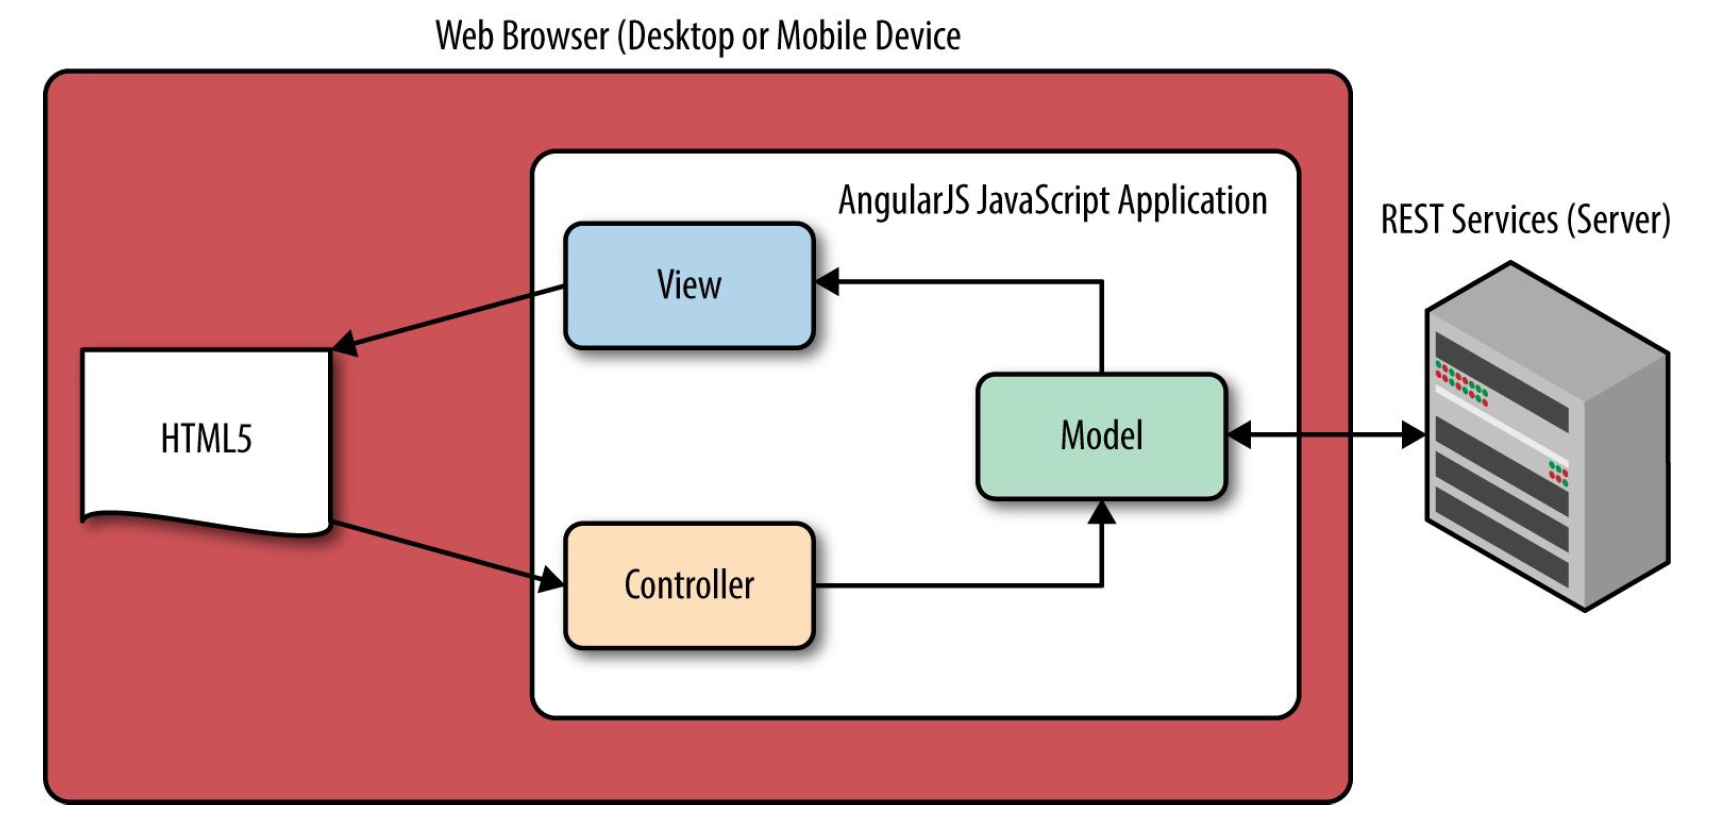
\includegraphics[width=0.9\textwidth]{Figures/MVC.png}\caption{MVC architektura v AngularJS}
\end{figure}

\subsubsection{Dvoucestný databinding}
Jedna z výhod frameworku AngularJS, kterou programátoři bezpochyby ocení, je dvoucestný databinding. Jedná se o automatickou synchronizaci mezi modelem a pohledem, kdy se změna jedné části automaticky projeví ve druhé. To umožňuje rychlou a pro prográmatora celkem nenáročnou synchronizaci mezi modelem v javascriptu a pohledem v HTML šabloně. Synchronizace se děje například pokud dorazí nová data nebo pokud uživatel provede nějakou akci. \cite{databinding}

\subsubsection{Dependency injection v AngularJS}
Dependency injection je návrhový vzor, ve kterém jsou závislosti definovány jako součást konfigurace aplikace. Díky této vlastnosti nemusí programátor ručně vytvářet použité závislosti. AngularJS načte a inicializuje všechny závislosti při spuštění aplikace, následně se stará o celý jejich životní cyklus. Programátor si tak jen napíše, kterou závislost chce ve své komponentě použít a pak už volá jen její metody.

Dependency injection díky snadnosti vložení závislostí usnadňuje testování, jelikož se snadno dají místo skutečných závislostí použít podvržené objekty.

Dependency injection se také používá v rámci Spring, v němž je jednou z klíčových součástí. Spring bude zmíněn v dalších kapitolách. \cite{LearningAngularjs}

\subsubsection{Základní proměnné}
V AngularJS se pro pojmenovávání objektů používá camel case. Jedná se o způsob psaní víceslovných názvů, kdy se pro oddělení slov nepoužívají mezery, ale místo toho každé další slovo začíná velkým písmenem.

Proměnné patřící rámci AngularJS začínají \$ nebo \$\$. Ty, jenž začínají dvěma dolary jsou, soukromé a programátor by k nim neměl vůbec přistupovat. Ty, jenž začínají jedním dolarem, se běžně používají. Níže je uvedeno pár hlavních.\\
\$location - poskytuje informace o aktuální URI na jednostránkové aplikaci, také svými funkcemi umožňuje přechod mezi stránkami.\\
\$http - slouží k volání http metod,\\
\$scope - propisuje proměnné do vybrané šablony.\\
\$rootscope - propisuje proměnné do všech šablon.

\subsubsection{Ukázka základního kontroléru}
Výpis kódu "Ukázka kontroléru v AngularJS"~popisuje základní kontrolér, jenž zavolá http metodu get nad URL http://test.com. Odpověď pak uloží do modelu na podstránce /game.
\\
\begin{lstlisting}[language=JavaScript, caption=Ukázka kontroléru v AngularJS]
var portRoyalApp = angular.module('portRoyalApp', [
    'rzModule',
    'portRoyalApp.gameModule'
    'portRoyalApp.jakykolivDalsiModul',]);

var gameCtrl = angular.module('portRoyalApp.gameModule', ['ngRoute']);

gameCtrl.controller('gameControler', function ($scope, $http) {
        $http.get('http://test.com').then
        (function (odpoved) {
            $scope.promennaDoSablony = odpoved.data;
        });
    })
    .config(['$routeProvider', function ($routeProvider) {
        $routeProvider.when('/game', {
            templateUrl: 'components/templates/game.html',
            controller: 'gameControler'
        });
    };
\end{lstlisting}
~\\
Na 1. - 4. se vytváří hlavní modul AngularJS do něhož se vkládají další moduly, z nichž je aplikace poskládaná. Například rzModule je modul stažený pomocí Node.js, přidávající posuvník. portRoyalApp.gameModule je modul vytvořený níže.\\
Na 6. řádku se vytváří modul pro hru, který v sobě obsahuje modul ngRoute pro pohyb v jednostránkové aplikaci.\\
Na 8. řádku se pro tento modul vytváří kontrolér, jenž si po pomocí Dependency Injection přidá 2 závislosti. \$scope a \$http.\\
Na 9. řádku se volá funkce get nad URL http://test.com poskytnutá \$http. Jedná se o asynchronní metodu, tudíž je její návratová hodnota slib zachycen funkci then. Tato funkce má jako vstupní parametr funkci, jenž zpracuje slib v momentě jeho naplnění\\
Na 10. - 12. řádku se zpracovává odpověď na get. Tato odpověď obsahuje hlavičku, http status a dalsí informace. V tomto případě je podstatný objekt jenž obsahuje, ten je uložený v objektu data. Ten se uloží do \$scope tak, že v ní vytvoříme nový objekt promennaDoSablony do nějž přiřadíme data.\\
Na 14. - 19.  řádku \$routeProvider konfiguruje pohyb na stránce. Je zde určeno, že pokud uživatel přejde na URI /game, zobrazí se mu šablona game.html, jenž má na starost gameControler. Ten se okamžitě při přechodu na tuto URI inicializuje. Tudíž spustí get metodu.


\subsection{Další technologie}

\subsubsection{Node.js}
Většinu problémů které řeší programátor v Javascriptu řešil už někdo před ním. Z tohoto důvodu by nebylo rozumné, aby programátor psal všechnu funkcionalitu sám. Je rozumější podívat se, zda už tato funkcionalita někde existuje. Proto vznikl Node.js. Node.js umožňuje programátorovi najít si funkcionalitu, a přidat ji do konfiguračního souboru. Po následném spuštění Node.js instalace se stáhnou požadované komponenty. Ty pak stačí pouze přidat pomocí Dependency injection.

Node.js také slouží jako spouštěč úloh, což znamená, že dokáže spouštět různé testovací rámce či fungovat jako server.

\subsubsection{Spring}
Spring je populární rámec pro vývoj J2EE aplikací s volnou licencí. Jeho první verze vyšla v červnu 2003 a od té doby značně nabyl na popularitě. 

Spring je označován jako kontejner, jelikož je modulární. V základu tudíž neumí téměř nic, až s přidáváním modulů získává další funkcionalitu. Ačkoli  přidávání dalších modulů komplikuje přípravu prostředí, je to výhoda, neboť následně na serveru běží pouze to, co je opravdu potřeba. Objekty přidané těmito závislostmi, případně programátorem, jež obsluhuje rámec Spring se nazývají Bean. Závislosti se přidávají přes Maven. V aplikaci Port Royal jsou použity například tyto moduly:
\begin{itemize}
	\item Hibernate - toto je implementace Java pesistance api, která slouží k namapování javovských entit na relační databázi. Následně pak zajišťuje komunikaci mezi databází a Springem.
	\item Spring Security - Spring Security poskytuje autentizaci a autorizaci uživatele.
	\item Tomcat plugin - Tomcat je open source webový server sloužící k nasazení aplikace. Implementuje většinu specifikace Java EE API. Tomcat je v této práci použit jako mavenovský plugin. Díky tomu není potřeba instalovat Tomcat server. Stačí pouze vytvořit spustitelný war soubor a následně spustit tento plugin mavenovským příkazem.
	\item AspectJ - Tento modul slouží k vytváření aspektu. Aspekty jsou funkce, které se volají nad větší skupinou různých objektů u nichž je potřeba stejné funkcionality. Použity jsou například pro autentizaci nebo logování příchozího dotazu, které se nemusí psát pro všechny třídy zvláště.
	\item spring websocket - Ve hře Port Royal, kterou hraje více hráčů najednou, je potřeba informovat hráče o akcích spoluhráčů. Každý hráč by měl tuto informaci dostat právě jednou a to co nejdříve. Toto zařídí websockety, které mají dvě URL. Jednu na níž se přihlásí všichni hráči ve hře, a druhou, na kterou hráči zasílají své akce. Pokud některý zašle svou akci na druhou URL budou o této akci informováni všichni hráči, kteří poslouchají na první URL.
\end{itemize}

\subsubsection{Maven}
Maven slouží ke kompilaci aplikace, ovšem nejen to. Umí spouštět testy či různé pluginy například výše zmíněný Tomcat plugin. Také slouží k přidávání závislostí, které se stejně jako pluginy definují do do souboru pom.xml. Maven tyto závislosti nebo pluginy pak sám stáhne. Toto jednak usnadňuje přidávání závislostí, jelikož programátor nemusí složitě stahovat různé a soubory stačí je pouze vypsat. Také usnadňuje přenos programu, jelikož stačí pouze přeposlat zdrojové kódy. O sestavení aplikace se všemi závislostmi se již dále postará maven.

\section{Typy testování}

%\subsection{Smysl testování software}
Testování dnes hraje při vývoji software důležitou roli. Organizace i vývojáři pochopili výhody testování hlavně u velkých aplikací, které se vyvíjejí a pak udržují mnoho let. U takovýchto aplikací mnohdy nelze s jistotou vědět, kde a jak se změny v kódu projeví. Pokud je ovšem určitá funkcionalita pokryta testy může se říci, že je tato funkcionalita splněna, jelikož to dokazují testy. A nejen to, pokud se bude kód upravovat, ví se, že testy pohlídají, aby byla původní funkcionalita zachována. Takto se předejde vytvoření chyb.

Ve výsledku tedy testy nejsou něco co by programátora zdržovalo. Právě naopak testy zabraňují výskytu chyb a ohlídají, aby měla aplikace požadovanou funkcionalitu. Takto testování šetří čas programátorů a peníze organizacím.

\subsection{Manuální oproti automatickým testům}
Testy se dají rozdělit na manuální a automatické. Manuálním testováním se rozumí když se tester vžije do role uživatele a ručně otestuje danou funkcionalitu oproti specifikaci. Tento typ testování je rychlý a jednoduchý, tudíž tester ani nemusí mít větší technické znalosti. Tyto testy jsou vhodné pro menší aplikace, které se nebudou měnit.

Problém nastává u větších a složitějších aplikací, v nichž nelze snadno a rychle zkontrolovat všechnu funkcionalitu manuálně. Této funkcionality je zde hodně. Proto jsou již potřeba automatické testy. Tyto testy sice trvá déle napsat, ovšem při několikanásobném opakování testu, jenž je potřeba po úpravách v aplikaci, jsou již automatické testy časově výhodnější.

Tato práce se zabývá automatickými testy.

\subsection{Test-driven development}
Klasický vývojový cyklus byl takový, že programátor dostal zadání, a to nastudoval. Následně napsal kód, trochu to lidově řečeno proklikal. Pokud se mu vše zdálo funkční, kód odevzdal. Pak bylo dále na testerovi, aby kód pořádně otestoval.

V dnešní době se však do popředí dostává Test-driven development neboli zkráceně už jen TDD. Tento přístup k vývoji předpokládá krátký vývojový cyklus neboli psaní software po menších částech. Vývojář praktikující TDD po obdržení a nastudování zadání nezačne psát implementaci zadání, ale nejprve vytvoří testy na požadovanou funkcionalitu. Tyto testy samozřejmě bez implementace požadované funkcionality budou hlásit chybu. Vytvoření požadované funkcionality je až další krok. Jak programátor tvoří požadovanou funkcionalitu, testy začínají procházet. Až v momentu, kdy všechny testy projdou, je vývoj dokončen. Programátor většinou při vývoji pouští pouze své testy, jelikož u větších systémů proběhnutí všech testů zabere několik minut. Všechny testy se tudíž většinou spouštějí až po dokončení práce pro potvrzení, že původní funkcionalita nebyla narušena.

\subsection{Úrovně testů}
Testy se také dají rozdělit na více úrovní podle toho, jak velký objem kódu pokrývají. U všech testů platí, že by se navzájem neměly ovlivňovat a měly by na sobě být nezávislé.

\subsubsection{Jednotkové testy}
Jednotkové testy jsou zaměřené na otestování funkcionality základních jednotek kódu. Většinou jedné funkce jedné třídy. Výhodou je, že tyto testy bývají rychlé a dobře se v nich identifikuje chyba. Jelikož neobsahují žádné další komponenty. Po napsání by měly zajistit, že daná část kódu plní svou funkcionalitu. Jedna funkcionalita může mít více testů pro různé vstupní parametry.

Při jednotkových testech v technologiích AngularJS a Spring se využívá Dependency injection. Komponenty, které využívá testovaný kód, se nahrazují podvrženými komponentami, díky čemuž není potřeba žádných závislostí a dá se nasimulovat různé chování ostatních komponent.

\subsubsection{Integrační testy}
Integrační testy propojují více komponentů. Testují, zda správně spolupracují a plní dohromady očekávanou funkcionalitu. Nevýhodou těchto testů je složitější odhalení chyby, pokud test selže, protože je nutno hledat chybu ve více komponentech. 

\subsubsection{End-To-End testy}
End-To-End testy simulují chování koncového uživatele v aplikaci. Tyto testy například kontrolují, zda se na stránce objeví určitý prvek, či zda se po kliknutí na něj provede očekávaná akce.

\subsection{Testovací technologie}
\subsubsection{Jasmine}
Jasmine je testovací rámec pro Javascript s otevřeným zdrojovým kódem. Má za cíl být nezávislý na ostatních rámcích či vývojářských prostředích. Snaží se také o snadno čitelnou syntaxi. Využívá se pro jednotkové testy nejen v prostředí AngularJS, ale i jiných technologiích založených na Javascriptu. Před každým testem se nejprve přidá testovaný modul, ten má spoustu závislostí. Pro tyto závislosti se vytvoří podvržené moduly. Takto se zajistí jednak, že se opravdu testuje pouze daný modul, ale také se takto dají nasimulovat různá vstupní data. Například určením hodnot, které budou vracet http odpovědi. Jasmine také umožňuje vytváření takzvaných špionů, kteří kontrolují, zda byla metoda zavolána, případně s jakými hodnotami.

\subsubsection{Protractor}
Protractor je end-to-end testovací framework pro AngularJS. Protractor spouští testy oproti skutečné aplikaci, která je již spuštěná na serveru. Spustí si prohlížeč, v němž simuluje chování skutečného uživatele. Protractor se na stránce naviguje pomocí http šablony, zde si nalezne elementy podle id, css stylu či modelu patřícímu AngularJS. S těmito elementy pak provádí akce nebo ověření jejich hodnoty oproti očekávané hodnotě. Protractor také umí počkat na načtené stránky, tudíž programátor nemusí zadávat pevnou dobu čekání. Což by jednak prodlužovalo běh testu, ale také by při zpoždění odpovědi serveru mohlo způsobit zahlášení selhání testu, jenž by ovšem bez mimořádného zpoždění prošel. \cite{TestingAngularApp}

\subsubsection{Karma}
Karma je spouštěč testu v Node.js. Využívá ho Jasmine i Protractor. Spouští prohlížeč, v němž běží testy.

\subsubsection{Jersey}
Jersey je testovací rámec vytvořen pro ověření správnosti serverových komponent. Testuje webové služby. Funguje to tak, že si Jersey rozjede svůj vlastní aplikační server s testovanými koncovými body. V této bakalářské práce se jako server používá Jetty, ovšem dá se použít i jiný server. Následně se volají tyto body, odpovědi serveru se pak porovnají s očekávanými. Pokud například vývojář dostane zadání aby vytvořil webovou službu, jež vrací nějakou hodnotu, snadno vytvoří test, kde pouze zavolá koncový bod podle zadání a porovná navrácenou hodnotu. U těchto testů je pouze zdlouhavější nastavení prostředí, následné testy se píší rychle a snadno.

\section{Obsah a funkcionalita aplikace}
Hra uvítá nově příchozího hráče uvítací stránkou na níž má možnost podívat se na statistiky hráčů. Dále se může přihlásit anebo registrovat. Po přihlášení přibude možnost vytvořit hru, do níž se mohou přihlašovat další hráči nebo se přihlásit do již vytvořené hry. Také zde přibude možnost přejít do administrace hráčů, pokud má hráč roli uživatele.

\subsection{Zkrácená pravidla hry}
Hra se dělí na dvě fáze. Nejprve aktivní hráč otáčí karty z kupky. Na stole se může objevit více druhů karet. Jsou zde karty lodí, za které obdrží hráč mince. Dále karty postav, jenž poskytují zvláštní schopnosti a poskytují vítězné body. Tyto karty si může hráč koupit pouze v případě pokud má dost mincí. Pak zde jsou expedice, ty se po otočení přesunou na zvláštní hromádku. Expedice poskytují vítězné body a také mince. Pokud má hráč postavy, jenž umožňují provést expedici, může je kdykoliv když je aktivní, vyměnit. Pak jsou ve hře ještě karty daní, při jejich otočení může hráč splňující určitou podmínku dostat mince, zároveň hráči mající 12 nebo více mincí musejí zaplatit polovinu svých mincí. Aktivní hráč otáčí karty tak dlouho, dokud se nerozhodne jednu z otočených karet vzít nebo dokud neotočí dva typy stejné lodi.

Následně začne druhá fáze v níž postupně může každý ze zbývajících hráčů kupovat karty ze stolu, pokud jsou zde nějaké k dispozici. Ovšem při tomto nákupu musí hráč, jenž karty otočil, zaplatit minci. Jakmile tato fáze skončí Stane se aktivním hráčem další hráč v řadě. Toto se děje do té doby dokud některý z hráčů nenasbírá 12 vítězných bodů

Celá pravidla je možno samozřejmě stáhnout ve hře nebo si je přečíst v příloze.

\subsection{Obsah a implementace stránky na vytváření hry}
V této kapitole je popsána stránka na vytváření hry, je zde použit posuvník k určení maximálního počtu hráčů. Při změně hodnoty na posuvníku se také změní hodnota modelu od AngularJS uvádějící maximální počet hráčů. Nad tímto modelem je použit \$watch, ten při pohybu posuvníku informuje serverovou část aplikace o změně.

Podobná kontrola probíhá při změně každé proměnné. Nazývá se dirty checking. Zajišťuje propsání změn mezi modelem a šablonou, případně mezi modely. Proto se doporučuje, aby počet proměnných na stránce nepřesáhl počet 5000.

\begin{figure}[H]
\centering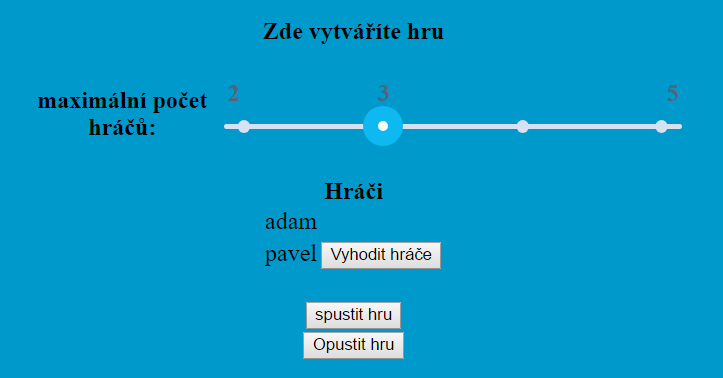
\includegraphics[width=0.95\textwidth]{Figures/gamecreationpage.png}\caption{Stránka na vytváření hry}
\end{figure}

\subsection{Obsah a implementace stránky s administrací}
Administrativní stránka je dostupná pouze uživatelům s rolí administrátora. Pokud by se na ni uživatel nějakým způsobem dostal, Spring Security stejně zablokuje všechny resty začínající /useradministration, což jsou resty provádějící akce na této stránce. Tudíž nedovolí provést žádnou neoprávněnou změnu. Stránka obsahuje seznam uživatelů seřazených podle přihlašovacího jména. Zde použito stránkování, kdy se na jednu stránku načte pouze deset uživatelů.

\begin{figure}[H]
\centering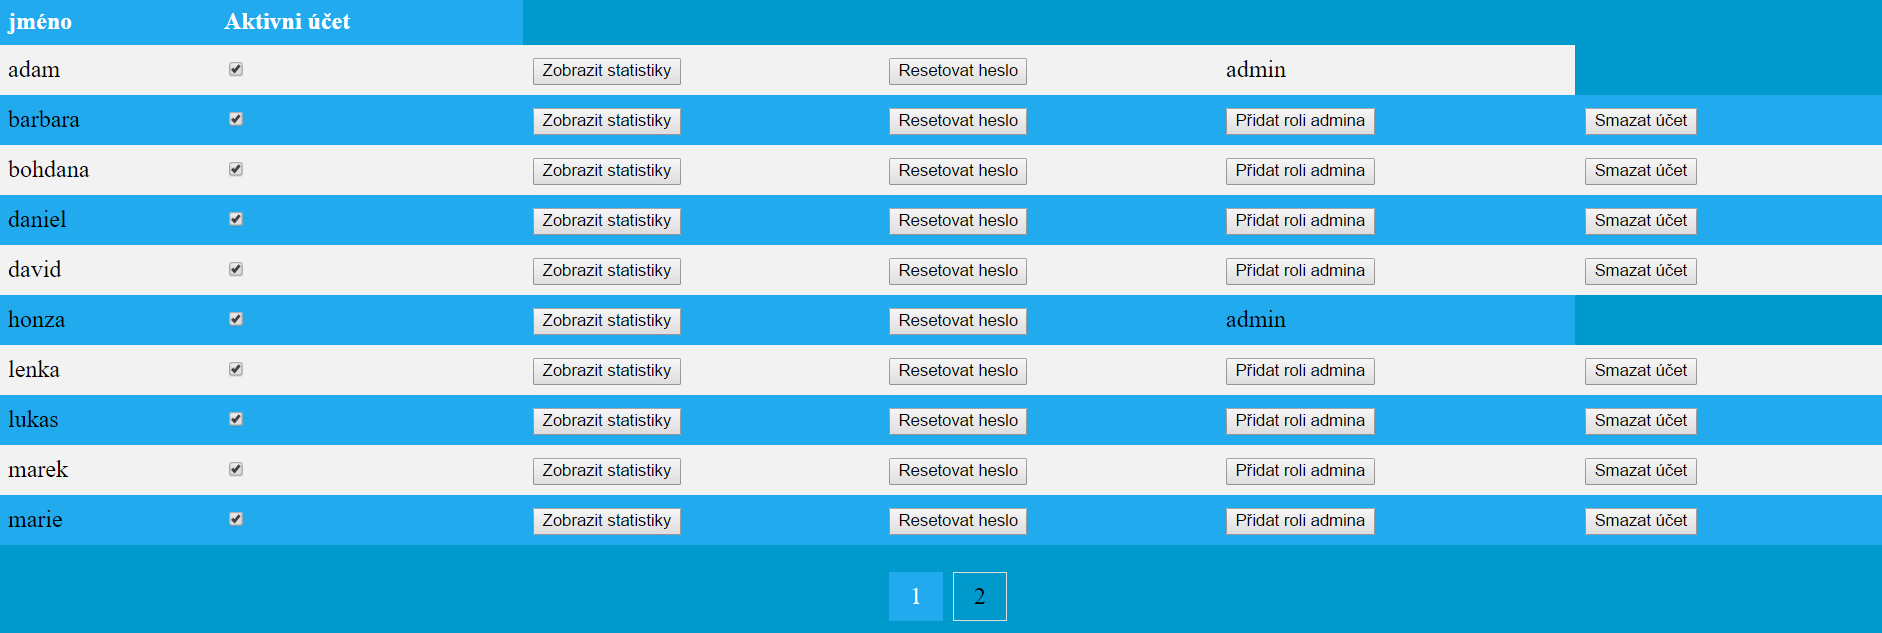
\includegraphics[width=0.95\textwidth]{Figures/administrationpage.png}\caption{Stránka administrace uživatelů}
\end{figure}

\subsection{Obsah a implementace stránky s hrou}
Hra je uložena v objektu, jenž obsahuje více stavů hry, které se postupně zobrazují, aby ukázaly akci aktivního hráče.
Pokud by zde bylo použito doptávaní se serveru v určitých intervalech, generovalo by to zbytečnou zátěž. Také by zde bylo zpoždění, jelikož by aktualizace stránky neproběhla okamžitě po akci. Nemluvě o riziku, že by se některá z akcí zobrazila několikrát, jelikož by bylo komplikované evidovat zda se daná akce již zobrazila.

Proto jsou zde použity websockety ty po zaslání akce na server aktualizují hráčům ve hře objekt se stavem hry okamžitě a právě jednou.
\begin{figure}[H]
\centering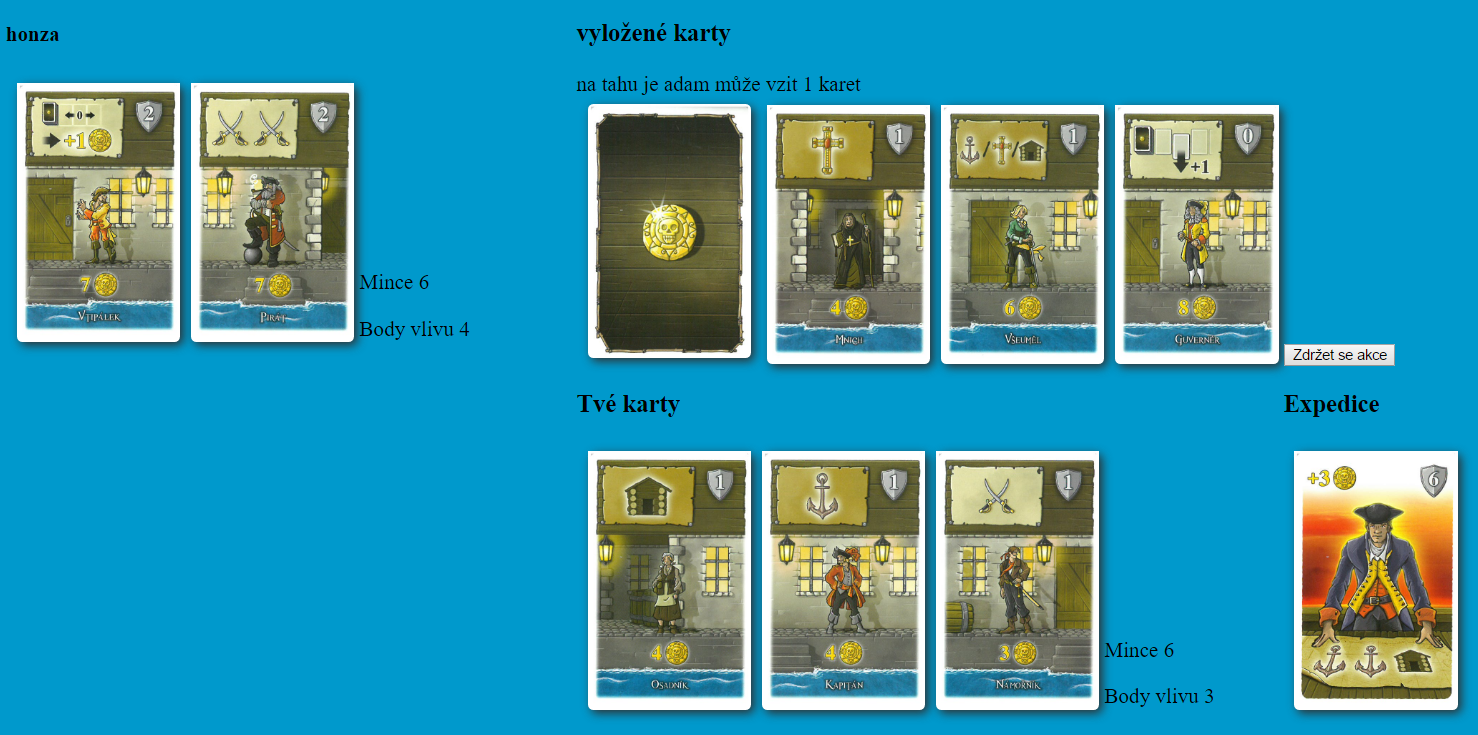
\includegraphics[width=0.95\textwidth]{Figures/gamepage.png}\caption{Stránka, na které se hraje hra}
\end{figure}


\section{Analýza použitých technologii}
Aplikace je vyvinuta ve Springu a jediné, co potřebuje je připojení do databáze, v níž si sama vytvoří tabulky pomocí Hibernate. Spring kontejner má v sobě dvě části.

Serverovou část napsanou v Javě jenž se stará o logiku aplikace a přistupující do databáze. Po nasazení na server obsluhuje webové služby. Tato část se nachází ve složce java. 

Klientskou část se nachází ve složce webapp, tato část obsahuje AngularJS. Při uživatelově vstupu do webové aplikace se celá tato část načte do prohlížeče. Po provedení akce se volá serverová část z níž si hráč zjišťuje potřebné informace.

Obě tyto části by se daly snadno oddělit do dvou serverů.

\subsection{Schema DB}
Hibernate po připojení do databáze vytvoří schéma na obrázku "Databázový model". Tento model se vytváří dle anotovaných entit. V této práci jsou použity přednastavené typy proměnných dle entit.
\\
\begin{figure}[H]
\centering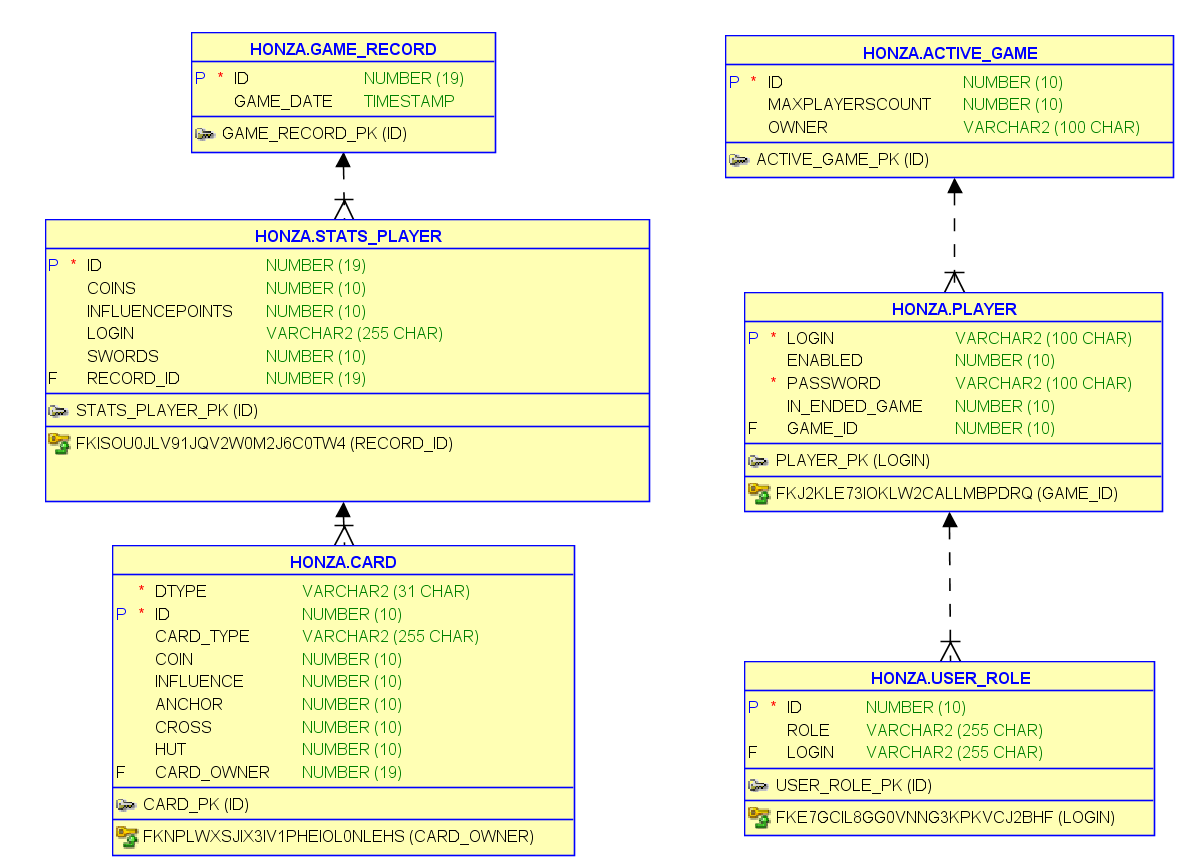
\includegraphics[width=0.95\textwidth]{Figures/DBmodel.png}\caption{Databázový model}
\end{figure}

\subsection{Node.js}
Pokud chce programátor přidat závislost přes Node.js, například posuvník. Je nejprve potřeba vyhledat závislost v tomto případě "angularjs-slider": "6.0.1", tato závislost se přidá do souboru bower.json, konkrétně do objektu dependencies. pak se ve složce s tímto souborem spustí příkaz "bower install". Tento příkaz do nakonfigurované složky stáhne nově přidanou závislost. Následně stačí pouze přidat nově stažený script do indexu a jeho modul do modulu AngularJS, jenž ho využívá. 

\subsection{Spring Security a Bcrypt}
Bezpečnost aplikace je řešená pomocí Spring Security, jenž po nakonfigurování blokuje URI na který uživatel nemá přístup.

Hesla v databázi nejsou samozřejmě uloženy pouze jako text. Pro heslo se při registraci uživatele vygeneruje hash pomocí Bcryptu. Tento hash je pak v databázi uložen místo hesla samotného. Při přihlašování Spring Security kontroluje, zda přihlašovací heslo odpovídá vygenerovanému hashi.

\subsection{Aspekty}
Spring podporuje aspekty, jenž se volají před každým zavoláním vybraných metod. V této podkapitole je ukázka aspektu nazvaná "Ukázka aspektu". Tento aspekt před každým zavoláním funkce z balíčku resource nastaví uživatele v Bean UsersProvider. Rozsáhlejší verze tohoto aspektu je použita v aplikaci. Pro Bean v rámci Spring je přednastaveno, že existuje jedna pro celý běh aplikace. U Bean UsersProvider je to v konfiguračním XML změněno. Vytváří se zvlášť pro každý http dotaz, jelikož na server přistupuje několik uživatelů zároveň. \\

\begin{lstlisting}[language=Java,label=src:Java, caption=Ukázka aspektu]
@Aspect
public class UserAspect {

    @Inject
    private UsersProvider usersProvider;

    @Before("execution (* vsb.cec0094.bachelorProject.resource.*.*(..))" +
            "&& !execution(* vsb.cec0094.bachelorProject.resource.StatsResource.*(..))")
    public void setUser() {
        String login = SecurityContextHolder.getContext().getAuthentication().getName();
            usersProvider.prepareUser(login);
    }
}
\end{lstlisting}
~\\
Na 1. řádku se anotacemi určí, že se jedná o Aspekt\\
Na 4. řádku je použita anotace Inject, touto anotací se říká v rámci Spring, aby do proměnné níže automaticky přiřadil Bean této třídy.\\
Na řádcích 7 až 9 se určí, že se funkce setUser má zavolat před každým voláním funkce třídy, jenž je v balíčku resource. Mimo třídu StatsResource, jenž Bean userProvider nepoužívá.\\
Na 10. řádku se pak z kontextu vyčte jméno přihlášeného uživatele.\\
Na 11. řádku se nastaví Bean userProvider.

\subsection{Komunikace mezi Spring a AngularJS}
Komunikaci mezi serverovou stranou aplikace v rámci Spring a AngularJS vždy začíná AngularJS zavoláním určitého koncového bodu, neboli URL přístupného klientským aplikacím. Koncové body obsluhuje Spring. To se děje v případě uživatelovy akce. Také v pozadí běží kontrola zda se uživatel nachází na správné URI v rámci aplikace, jenž se v pravidelných intervalech ptá na jaké URI by se měl uživatel nacházet a kontroluje, zda na ní opravdu je. To se děje pro případ, že by uživatel ve hře přešel třeba tlačítkem zpět do statistik či vypnul prohlížeč. Po znovu-spuštění aplikace je ho potřeba přesměrovat na URI s hrou. Na uvítací stránce a na stránce, kde běží hra, jsou použity websockety, pro chat a aktualizování hry.

\subsection{Websockets}
Zde je ukázka nastavení websocketu pro chat, jenž je na úvodní stránce. Websockety je nutno nastavit jak na straně serveru (Spring), tak na straně klienta (AngularuJS). Následně to funguje tak, že se klienti přihlašují k odběru zpráv na server. V momentě kdy chce některý z klientů poslat zprávu všem ostatním klientům, odešle ji na server. Ten ji následně rozešle všem naslouchajícím klientům.

\subsubsection{Serverová strana}
Serverová strana websocketu se nastavuje v rámci Spring. Je zde nutno přidat závislosti ze skupiny "org.springframework"~konkrétně "spring-messaging"~a "spring-websocket"

V XML konfiguraci se nastaví, že se uživatelé mohou připojovat k websocketům na URI "/chat". Na URI "/messages"~je pak ještě možno přihlásit se k odběru zpráv.\\
\begin{lstlisting}[language=XML, caption=XML konfigurace websocketu]
<websocket:message-broker application-destination-prefix="/port-royal/">
    <websocket:stomp-endpoint path="/chat">
        <websocket:sockjs/>
    </websocket:stomp-endpoint>
    <websocket:simple-broker prefix="/messages"/>
</websocket:message-broker>
\end{lstlisting}

V Javě je nutno vytvořit funkci, jenž zpracovává příchozí zprávy. V této kapitole je ukázka kódu nazvaná "Implementace websocketu v javě"~.Na prvním řádku se určí URI, pro příchozí zprávy. Na druhém řádku se určí URI na které jsou odběratelé, jenž všichni dostanou zpracovanou zprávu. Dále je jen zpracování a odeslání zprávy.\\

\begin{lstlisting}[language=Java, caption=Implementace websocketu v javě]
@MessageMapping("/sendMessage")
@SendTo("/messages")
public Message receive(Message message) {
    return message;
}
\end{lstlisting}

\subsubsection{Klientská strana}
Klientská část aplikace se nastavuje v AngularJS. Je zde ukázka kódu pod názvem "Použití websocketu na straně klienta", pro níž je nutno mít závislosti "sockjs" a "stomp-websocket", které se přidávají přes Node.js.

Jsou zde 3 asynchronní funkce. Nejprve je nutno se připojit na serverový koncový bod funkci connect. Konkrétně se zde připojuje na URI "/port-royal/chat". 

Pak je možno začít odebírat zprávy funkcí subscribe, jež vypíše do konzole všechny příchozí zprávy. Také je možné odeslat předem vytvořenou zprávu funkcí send.
\\
\begin{lstlisting}[language=JavaScript, caption=Použití websocketu na straně klienta]
var client;      
function connect() {
    var socket = new SockJS('/port-royal/chat');
    client = Stomp.over(socket);
    client.connect();
};
function subscribe() {
    client.subscribe("/messages", function (message) {
        var body = JSON.parse(message.body);
        console.log('message was recived', body);
    });
};
function send () {
    client.send("/port-royal/sendMessage", {}, JSON.stringify(
        {'text': 'test message',
        'author': 'Honza Cech'}
    ));
};
\end{lstlisting}

\subsection{Architektura aplikace}
Všechny spuštěné hry na serveru jsou uloženy v hash mapě objektu GamesHolder, ta v sobě obsahuje pro každou hru GameManipulator. Pokud si uživatel vyžádá svou hru, vrátí se mu GameManipulator s id jeho hry. Aktuální hra je uložena v objektu currentGame, ten je třídy Game, jež je popsána dále v této kapitole. Objekt currentAction informuje, zda má být nějaká karta zvýrazněna.

GameManipulator také obsahuje dva listy gamesToShow a actionsToShow. Tyto listy spolu obsahují již zahrané stavy hry (objektů v obou listech bude stejný počet, jelikož ke každému objektu hry je jeden objekt, jenž obsahuje informaci zda, je nutno něco zvýraznit). Tyto stavy jsou potřeba, pokud je nutno zvýraznit nějakou akci hráče (například pokud hráč kupuje kartu ze stolu). Nejprve se mu zobrazí historický stav, kdy byla nově zakoupená karta ještě na stole se zvýrazněnou kupovanou kartou. Následně se mu zobrazí stav, kdy má již koupenou kartu ve svých kartách se zvýrazněnou koupenou kartou. Až nakonec se zobrazí aktuální hra bez žádných zvýrazněných akcí.

\begin{figure}[H]
\centering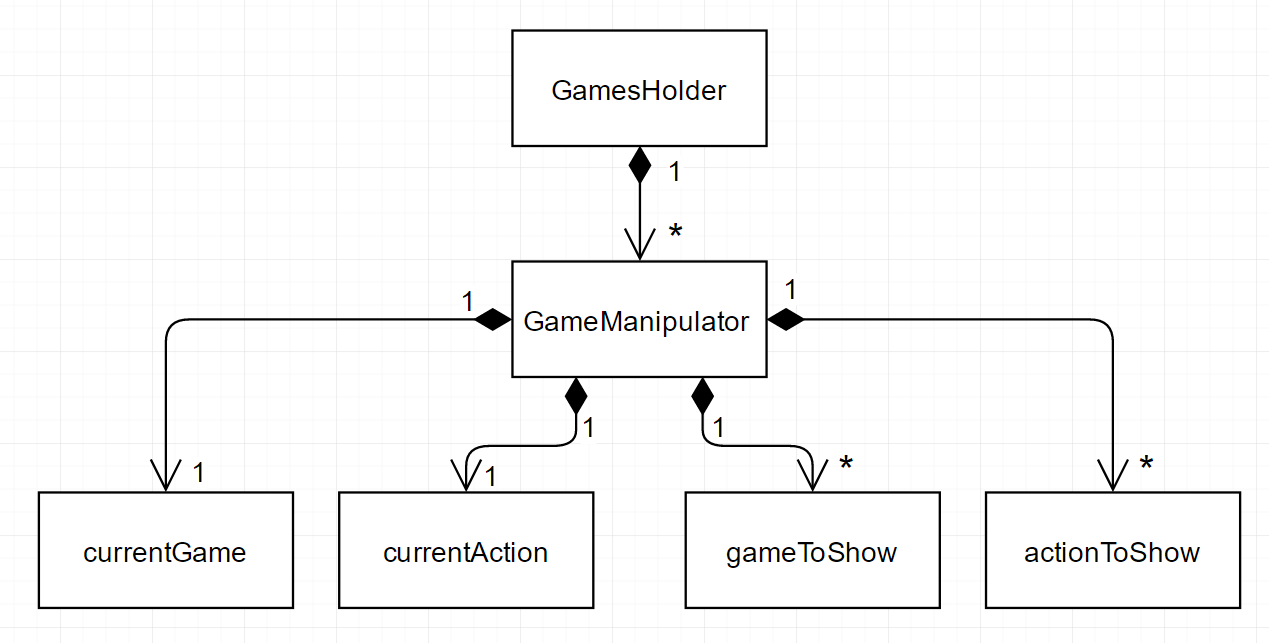
\includegraphics[width=0.95\textwidth]{Figures/GameManipulator.png}\caption{Model uložení her na serveru}
\end{figure}

Obrázek~"Model hry"~popisuje objekt Game, v němž jsou uloženy informace o stavu hry. Game obsahuje 4 typy objektů, které reprezentují různá místa, kde se karty mohou nacházet. Tyto objekty si následně mezi sebou vyměňují karty dle uživatelových akcí.

\begin{figure}[H]
\centering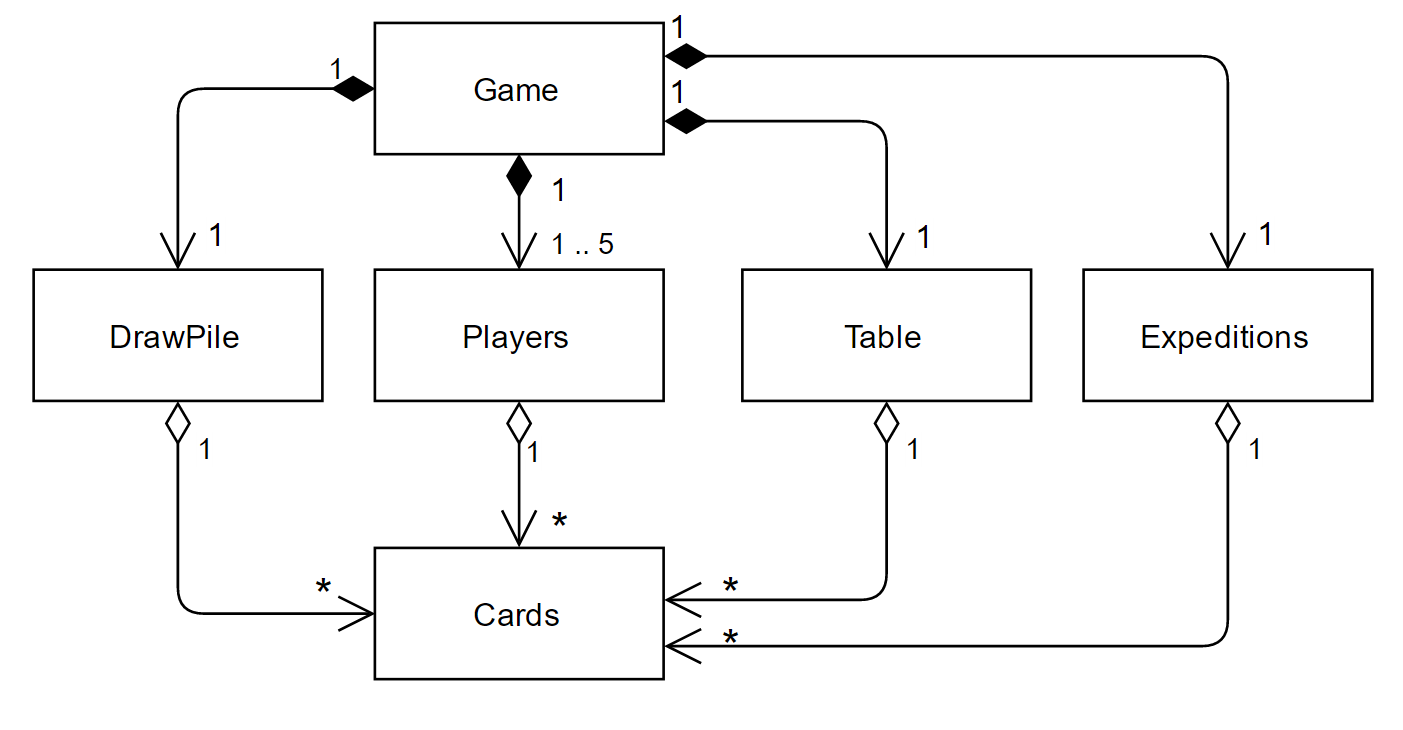
\includegraphics[width=0.95\textwidth]{Figures/Game.png}\caption{Model hry}
\end{figure}

Příchozí dotazy na server jsou nejprve odchyceny Bean UserAspect, ta zjistí z kontextu login uživatele. Poté provede dotaz do databáze, ze které si vytáhne potřebné informace o uživateli. Pokud zjistí, že je uživatel ve spuštěné hře, vytáhne si také z Bean GamesHolder vybranou hru. Následně dotaz zpracovává vybraná třída z balíčku resource. Hru a potřebné informace ji poskytuje UserProvider. Pokud se jedná o akci vyžadující přístup do databáze, využívá k ní vybraná resource třída některý z objektů v balíčku dao. Pokud se mění stav spuštěné hry, resource třída zadá instanci GameManipulator pokyn pro vykonání akce.

\begin{figure}[H]
\centering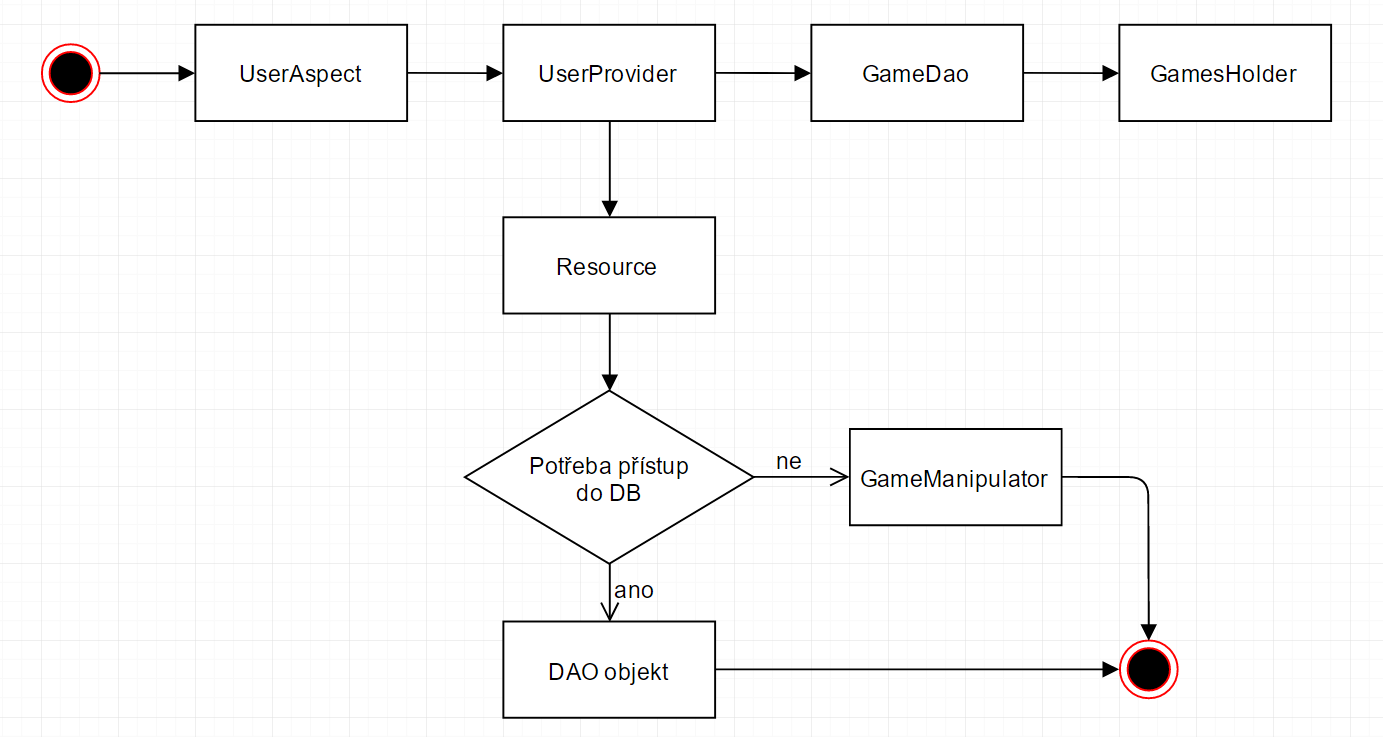
\includegraphics[width=0.95\textwidth]{Figures/RequestFlow.png}\caption{Zpracování dotazu}
\end{figure}

\section{Analýza a implementace testu}

\subsection{Jasmine}
Jasmine testy se spouštění přes Node.js příkazem "npm test"~ve složce se souborem package.json., v němž je uvedena cesta ke konfiguračnímu souboru karmy. V tomto souboru jsou uvedeny cesty k testům a pluginy pro spuštění prohlížeče, v němž se testy jeden po jednom spouštějí. 

Samozřejmě, že také existuje software jako například Karma plugin pro InteliJ IDEA jenž umožňují spustit testy jedním kliknutím ve vývojovém prostředí.

\subsubsection{Ukázkový test}
Ukázkový kód v této kapitole je test, jenž ověří, zda se po zavolání funkce login od loginService, skutečně zavolá backendGateway. BackendGateway komunikuje ven z aplikace. Test také zkontroluje zda, funkce vrátí login nově přihlášeného uživatele.
\\
\begin{lstlisting}[language=JavaScript, caption=Ukázka testu pomocí Jasmine]
describe('example test for portRoyalApp.loginService', function () {
    var $q, $rootScope, loginService, backendGateway;

    beforeEach(function () {
        module('portRoyalApp.loginService');
        module({
            'backendGateway': jasmine.createSpyObj('backendGateway', ['get', 'post'])
        });

        inject(['$q', '$rootScope', 'loginService', 'backendGateway',
            function (_$q_, _$rootScope_, _loginService_, _backendGateway_) {
                $q = _$q_;
                $rootScope = _$rootScope_;
                loginService = _loginService_;
                backendGateway = _backendGateway_;
            }]);
    });

    it('should login user and return his login when login is called', function () {
        //prepare
        var loggedUser;
        var userName = 'MOCKED_USERNAME';
        var password = 'MOCKED_PASSWOED';
        var expectedConfig = {
            params: {
                username: userName,
                password: password
            },
            ignoreAuthModule: 'ignoreAuthModule'
        };
        backendGateway.get.and.returnValue($q.resolve({data: 'MOCKED_USER_FROM_BACKEND'}));
        backendGateway.post.and.returnValue($q.resolve());
        //test
        loggedUser = loginService.login(userName, password);
        //validation
        $rootScope.$digest();
        expect(backendGateway.post).toHaveBeenCalledWith('LOGIN_URL', '', expectedConfig, false, true);
        expect(loggedUser).toEqual($q.resolve('MOCKED_USER_FROM_BACKEND'));
    });
});
\end{lstlisting}
~\\
Na 1. řádku se určuje, že se jedná o test pomocí describe, jenž shlukuje Jasmine testy. První parametr je popis skupiny testů, druhý je funkce se skupinou testů.\\
Na 2. řádku se vytváří proměnné, jenž se budou využívat.
Na 4. až 17. řádku je funkce beforeEach, jenž se spouští před každým testem v této skupině. V této funkci se nejprve přidává testovaný modul. Následně jeho závislosti, v tomto případě se jedná pouze backendGateway. Zde se nepřidává skutečný modul, ale pouze podvržený objekt, který má dvě funkce get a post, obě bez implementace. Po přidání modulů se na řádcích 10 až 15 zpřístupní z modulů objekty, jenž se budou dále používat.\\
Na 19. řádu začíná test. To udává funkce it, jenž má 2 vstupní parametry. První parametr je popis jehož jmenná konvence vypadá takto: it(should "očekávané chování~"when"~co se děje/jaké jsou vstupní podmínky). Druhý parametr je funkce s testem.\\
Na 21. až 30. řádku se připravují pomocné proměnné pro test.\\
Na 31. a 32. řádku se určují návratové hodnoty funkcí podvržených objektů. Zde by bylo možno také napsat celou novou funkci, jenž by se provedla po zavolání. Použitím callFake() místo returnValue().\\
na 34. řádku se zavolá testovaná funkce.\\
Na 36. řádku se vyvolá dirty checking (zmíněn v kapitone~4.2). Ten je použit pro vyhodnocení asynchronních metod.\\
Na 37. řádku se zkontroluje, zda byla opravdu zavolána backendGateway se správnými parametry pro přihlášení.\\
Na 38. řádku se provádí kontrola vrácené hodnoty.\\

\subsection{Protractor}
Protractor se pouští stejně jako Jasmine přes Node.js ve složce se souborem package.json. Ovšem příkazem "npm run protractor". V souboru package.json. je cesta ke konfiguračnímu souboru Protractoru, v tom se nastavuje na jaké URL je spuštěn testovaný server nebo v jakém prohlížeči se mají testy spouštět. 

Kód v této kapitole s názvem "Ukázkový Protractor test"~je  test, který zkontroluje, zda se uživatel úspěšně přihlásí.
\\
\begin{lstlisting}[language=JavaScript, caption=Ukázkový Protractor test]
describe('examle login test', function () {
    it('should login user', function () {
        browser.get('http://localhost:8090/port-royal/#!/login');
        browser.ignoreSynchronization = true;

        var pageTittle = element(by.id('loginLabel'));
        expect(pageTittle.getText()).toMatch('Zde se muzete prihlasit');

        element(by.model('userName')).sendKeys('honza');
        element(by.model('password')).sendKeys('heslo');
        element(by.id('loginButton')).click();
        browser.sleep(2500);

        expect(browser.getLocationAbsUrl()).toMatch("/welcome");
        pageTittle = element(by.css('.mailLabel'));
        expect(pageTittle.getText()).toMatch('Vitej pirate honza');
    });
});
\end{lstlisting}
~\\
Na 3. a 4. řádku se nastavuje prohlížeč. Nejprve se mu určí adresa, na níž má test začínat. Protractor v základním nastavení umí poznat načtení stránky a počkat na něj. Tuto schopnost je nutno vypnout, protože v pozadí je spuštěna v nekonečné smyčce funkce, jež kontroluje, zda je uživatel na správné stránce.\\
Na 6. a 7. řádku se děje kontrola nadpisu na přihlašovací stránce. Protractor umí vyhledávat prvky mnoha způsoby, zde se tak děje pomocí id elementu. Následuje porovnání očekávaného textu nadpisu se skutečným.\\
Na 9. až 12. řádku probíhá přihlášení. Protractor nalezne elementy podle modelu od AngularJS a vyplní je hodnotami. Poté se klikne na tlačítko přihlášení. Jelikož je automatické čekání na~načtení stránky vypnuté je nutno pevně nastavit dobu po níž bude prohlížeč čekat na načtení stránky.\\
Na 14. řádku se provádí kontrola, zda po přihlášení došlo k přesměrování na uvítací stránku.\\
Na 15. a 16. řádku opět probíhá kontrola titulku stránky, zde se ovšem titul nalezne pomocí css třídy.

\subsection{Jersey}
Jersey testy jsou testy psané v rámci Spring. Testy v rámci Spring se spouštějí přes maven příkazem test a také automaticky při sestavování aplikace. Aby se testy spustily musí být ve složce src/test a jejich název musí odpovídat jednomu ze vzorců níže.
\begin{itemize}
	\item "**/Test*.java"
	\item "**/*Test.java"
	\item "**/*Tests.java"
	\item "**/*TestCase.java"
\end{itemize}

\subsubsection{ukázkový test}
Všechny testy použité ve hře Port Royal se dědí z BaseJerseyTest, jenž je uveden v ukázce kódu "BaseJerseyTest". BaseJerseyTest dědí z JerseyTest, což je třída ze závislosti org.glassfish.jersey.test. Přepisuje její funkci configure, která nastavuje testy. Přepsaná metoda používá vlastní  konfiguraci a sadu Bean uložené v XML souboru jersey-context-test.xml.
\\
\begin{lstlisting}[language=Java, caption=BaseJerseyTest]
@ContextConfiguration(locations = {"classpath:/jersey-context-test.xml"})
public abstract class BaseJerseyTest<T> extends JerseyTest {

  @Override
  protected Application configure() {
     ResourceConfig resourceConfig = new ResourceConfig(getResourceClass());
     resourceConfig.property("contextConfigLocation", "classpath:/jersey-context-test.xml");
     resourceConfig.register(new AbstractBinder() {
        @Override
        protected void configure() {
           bindServices(this);
        }
     });
     return resourceConfig;
  }
  
  protected abstract void bindServices(AbstractBinder binder);

  protected abstract Class<T> getResourceClass();
}
\end{lstlisting}

Následně se již píší konkrétní testy. Například test ve výpisu "Konkrétní Jersey test" kontroluje, zda URI "/play/getMyGame"~skutečně vrací objekt obsahující hráčovu hru.
\\
\begin{lstlisting}[language=Java, caption=Konkrétní Jersey test]
@RunWith(SpringJUnit4ClassRunner.class)
public class PlayGameResourceTest extends BaseJerseyTest<PlayGameResource> {
    @Inject
    private PlayGameResource playGameResource;
    @Inject
    private UsersProvider usersProvider;
    private GameManipulator expectedGame;

    @Override
    protected void bindServices(AbstractBinder binder) {
        binder.bind(playGameResource).to(PlayGameResource.class);
    }
    @Override
    protected Class<PlayGameResource> getResourceClass() {
        return PlayGameResource.class;
    }
    
    @Before
    public void setUp() throws Exception {
        super.setUp();
        MockitoAnnotations.initMocks(this);
        expectedGame = new GameManipulator();
        expectedGame.setId(666);
        when(usersProvider.getGameManipulator()).thenReturn(expectedGame);
    }
    
    @Test
    public void testGetMyGame() {
        //test
        final Response response = target("/play/getMyGame")
                .request()
                .get();
        GameManipulator game = response.readEntity(GameManipulator.class);
        //validation
        assertEquals(Response.Status.OK.getStatusCode(), response.getStatus());
        assertEquals(expectedGame, game);
    }
}
\end{lstlisting}
~\\
Na 1. řádku je potřeba nastavit spouštěč testů.\\
Na 2. až 16. řádku se připravují proměnné a konfiguruje testovací třída přepsáním abstraktních metod pro konkrétní test.\\
Na 18. až 25 řádku se dokončuje nastavení prostředí. Přidaná Bean usersProvider nemá svou implementaci. V XML konfiguraci je místo ní nastaven podvržený objekt. Na 24. řádku se určuje co má vrátit jeho metoda getGameManipulator.\\
Na 28. až 37. řádku probíhá samotný test. Nejprve se zavolá http metoda na testovanou URI nad objektem target, ten je zděděn z předka JerseyTest. Následně se ověří, zda vrácený objekt odpovídá očekávanému.

\section{Závěr}
V praktické části této práce vznikla webová hra Port Royal. Tato hra se hraje na centrálním serveru, umožňuje správu uživatelských účtů. Také vytváří a eviduje statistiky odehraných her. Pro vytvořenou hru následně vznikly testy, které ji testují několika způsoby na klientské i serverové části. Práci hodnotím pozitivně, jelikož jsem se naučil mnoho moderních technologií používaných i v praxi při vývoji webových aplikací. Následně jsem si zkusil jejich praktické použití na rozsáhlejším projektu.

\subsection{Co bych dělal jinak}
Při vývoji byly použity konfigurace aplikace pomocí XML souborů. To se nakonec ukázalo jako nevhodné neboť se v dnešní době do popředí dostává konfigurování pomocí anotací. Tudíž většina návodů byla pro tuto aplikaci nevhodná.

\subsection{Jak by se dala aplikace vylepšit}
Spuštěná hra je uložena v paměti běžícího serveru. Při restartu serveru tudíž dojde i k restartu hry. Tento nedostatek by se dal odstranit průběžným ukládáním hry do databáze.

Pro přidání Jersey testů bylo nutno vytvořit nový kontext. Do tohoto kontextu se bohužel nepodařilo přidat websockety. Tudíž jsou v aplikaci dva kontexty jeden s websocketami a druhý se vší logikou. Websockety ve hře tudíž pouze informují aby si hráč stáhl nový stav hry, z druhého kontextu, místo toho aby nový stav hry samy odeslaly. 

\newcommand{\registerToBib}[4]
{
\bibitem{#1}
	{\bf #2}
	{[cit. #3].}
	{\em Dostupne z: #4}
}

\begin{thebibliography}{99}
\bibitem{test}
	{RUEBBELKE, Lukas a Brian FORD.}
	{AngularJS in action}
	{AngularJS in action. ISBN 1617291331.}

\bibitem{test2}
	{docs.angularjs.org}
	{[online].[cit.2017-06-01].}
	{Dostupné z: https://docs.angularjs.org}
	
\bibitem{test3}
	{Roy Thomas Fielding}
	{Architectural Styles and
the Design of Network-based Software Architectures}
	
	
	\registerToBib{coJeAngular}{angularjs}{2017-01-04}{https://docs.angularjs.org/guide/introduction}		
	\registerToBib{SPA}{nevim}{2017-01-04}{https://neoteric.eu/single-page-application-vs-multiple-page-application}
	\registerToBib{nikde}{taka sablona}{2017-01-04}{https://www.zdrojak.cz/clanky/zaciname-s-angularjs/}
	\registerToBib{databinding}{angularJS.org}{2017-02-04}{https://docs.angularjs.org/guide/databinding}
	\registerToBib{WebServices}{Oracle documentation}{2017-06-04}{https://docs.oracle.com/javaee/7/tutorial/webservices-intro001.htm\#GIJVH}
	\registerToBib{RESTWebServicesOracle}{Oracle documentation}{2017-06-04}{https://docs.oracle.com/javaee/7/tutorial/webservices-intro002.htm\#GIQSX}
	\registerToBib{RESTWebServicesOracle2}{Oracle documentation}{2017-06-04}{http://docs.oracle.com/javaee/6/tutorial/doc/gijqy.html}
	\registerToBib{RESTInterface}{Tutorialspoint}{2017-06-04}{https://www.tutorialspoint.com/restful/restful\_introduction.htm}
	\registerToBib{LearningAngularjs}{Williamson, Ken.}{2017-07-04}{Learning Angularjs: A Guide to Angularjs Development. Sebastopol, CA: O, 2015.}
	
	\registerToBib{TestingAngularApp}{Jesse Palmer}{2017-08-04}{Testing Angular Appliacction Cover Angular 2. 2016}
	
\end{thebibliography}

\appendix
\section{Instalace a spuštění aplikace}

\subsection{Instalace}
Aby mohla být aplikace spuštěna je nutno mít nainstalovaný Maven a Node.js. Také je potřeba mít k dispozici Oracle databázi.

Pokud jsou tyto prerekvizity splněny je možno začít s instalací. Nejprve je nutno nastavit připojení do databáze nastavením proměnných username, password a url. Ty se nastavují v souborech jdbc.properties, jenž se nacházejí na cestě \textbackslash src\textbackslash main\textbackslash resources a \textbackslash src\textbackslash test\textbackslash resources.

Následně je nutno stáhnout závislosti pro část v AngularJS. To se provede v příkazovém řádku příkazem "npm install" na cestě \textbackslash src\textbackslash main.

\subsection{Spuštění}
Pro spuštění aplikace je nutno mít volný port 8090. Poté stačí zadat v příkazovém řádku nad hlavním adresářem práce příkaz "mvn clean install tomcat7:run". Stahování všech závislostí může chvíli trvat. Po doběhnutí tohoto příkazu bude aplikace přístupná na adrese "http://localhost:8090/port-royal/".

Jasmine testy se spouštějí v příkazovém řádku na cestě \textbackslash src\textbackslash main příkazem "npm test". Protractor testy na stejné cestě příkazem "npm run protractor", tyto testy ovšem potřebují mít spuštěnou aplikaci na aplikačním serveru.

Pro spuštění Jersey testu se do příkazové řádky musí v hlavním adresáři napsat "mvn test".

\section{Přílohy ve formě CD}
Součástí práce je CD s zdrojovými kódy a s teoretickou práci v elektronické podobě.
\end{document}
